% contribuutions



% \begin{figure}[tbph]
% \centering
% 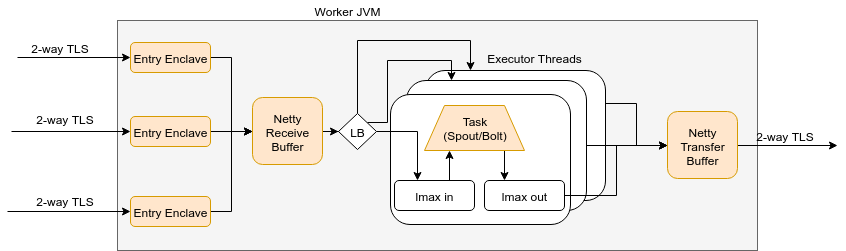
\includegraphics[width=.5\linewidth]{resource/img/ch_intro/stormsgx.png} %Include graphic at 1=100 \% linewidth vs textwidth as it will size if put in columns. Textwidth wont resize in columns
% \caption{Storm SGX architecture}
% \label{fig:sgx_arch}
% \end{figure} 

In this thesis we provide a framework for the systematic validation of the existing security metrics body of knowledge. In doing so we endeavour not only to survey the current state of the art, but also to create a common platform for future research in the area to be conducted. 

We  then  demonstrate  the  utility  of  our  framework  through  the  evaluation  of  leading security metrics against a reference set of system models we have created.  We investigate how  to  calibrate  security  metrics  for  different  use  cases  and  establish  a new methodology  for security metric benchmarking. To support automated and repeatable testing, each metric is implemented as an independent module containing the computation logic. These metric implementations can then be called directly from an embedded library, accessed through a benchmark test with standard interfaces and return types, or managed with a container orchestration engine. Each test has an associated specification which is used to configure dependencies and tuning parameters for execution. 
Specifically, we:
\begin{itemize}
\item Provide a methodology for calibrating security metrics against a fixed baseline and demonstrate isolation criteria for benchmark regimens
\item  Implement several distinct execution paradigms for different use cases 
\item Describe validation mechanisms available through increasingly sophisticated modeling and simulation extensions
\end{itemize}

We further explore the research avenues unlocked by automation through our concept of an API driven S-MaaS (Security Metrics-as-a-Service) offering. We review our design considerations in packaging security metrics for programmatic access, and discuss how various client access-patterns are anticipated in our implementation strategy. Using existing metric processing pipelines as reference, we show how the simple, modular interfaces in S-MaaS support dynamic composition and orchestration. We anticipate consumers will fall into one or more of the following access patterns:
\begin{itemize}
\item \textbf{R\&D}: A clean environment for developing and testing metrics.
\item \textbf{Reporting}: Measurements are pushed to persistent storage or pulled from a client into a structured format for charting and analysis. 
\item \textbf{Batch}: Client asynchronously submits a collection of inputs to calculate metrics for, with the target use-case being dataset preparation for supervised learning.
\item \textbf{Stream}: Client defines dependency graphs amongst metrics and connects these topologies to data sources for continuous stream processing.  
\end{itemize}


Next we review aspects of our framework which can benefit from optimization and further automation through machine learning. First we create a dataset of network models labeled with the corresponding security metrics. By training classifiers to predict security values based only on network inputs, we can avoid the computationally expensive attack graph generation steps. We use our findings  from this simple experiment to motivate our current lines of research into supervised and unsupervised techniques such as network embeddings, interaction rule synthesis, and reinforcement learning environments. 

Finally, we examine the results of our case studies. We summarize our security analysis of a large scale network migration, and list the friction points along the way which are remediated by this work. We relate how our research for a  large-scale performance benchmarking project has influenced our vision for the future of security metrics collection and analysis through DevOps automation. We then describe how we applied our framework to measure the incremental security impact of running a distributed stream processing system inside a hardware trusted execution environment.

This work begins to develop the foundation for a repeatable, extensible security analytics benchmarking framework, allowing existing and proposed metrics to be implemented in uniformly accessible ways and tested against standard reference models. Through automation we lower the barrier of entry for future research and expand accessibility to client applications not currently integrating security metrics in practice. 

% To summarize:
% \begin{itemize}
% \item We created a rapid prototyping and integration environment for security metrics. 
% \item We developed a reference data set for validating security metrics across different topologies and scales.
% \item We implemented benchmark tests in a widely adopted open source benchmark test suite to reach the largest audience. 
% \item We developed S-MaaS, a scalable deployment system where metrics are microservices.
% \item We enhanced S-MaaS automation using a variety of machine learning applications.
% \item We present case studies and lessons learned as evidence our framework is practical and effective.

% \end{itemize}






